	\begin{frame}
	\frametitle{День 5. 22 августа}
	\framesubtitle{д.р. Кичкинекол Джалпаккольский~--- м.н. под моренным валом пер. Джалпаккол Северный} % Optional subtitle
	\begin{columns}[c] % The "c" option specifies centered vertical alignment while the "t" option is used for top vertical alignment
		\begin{column}{0.45\textwidth} % Left column width
			\begin{itemize}
				\item Мємі
				\item Прохождение каменного лабиринта
				\item Гроза
				\item Прошли \textbf{5.8} км
				\item ЧХВ: 3:56
				\item Набор/сброс: \textcolor{darkred}{\textbf{+620}}/\textcolor{darkblue}{\textbf{-0}}~м
			\end{itemize}
			
		\end{column}
		\begin{column}{0.5\textwidth} % Right column width
			\centering
			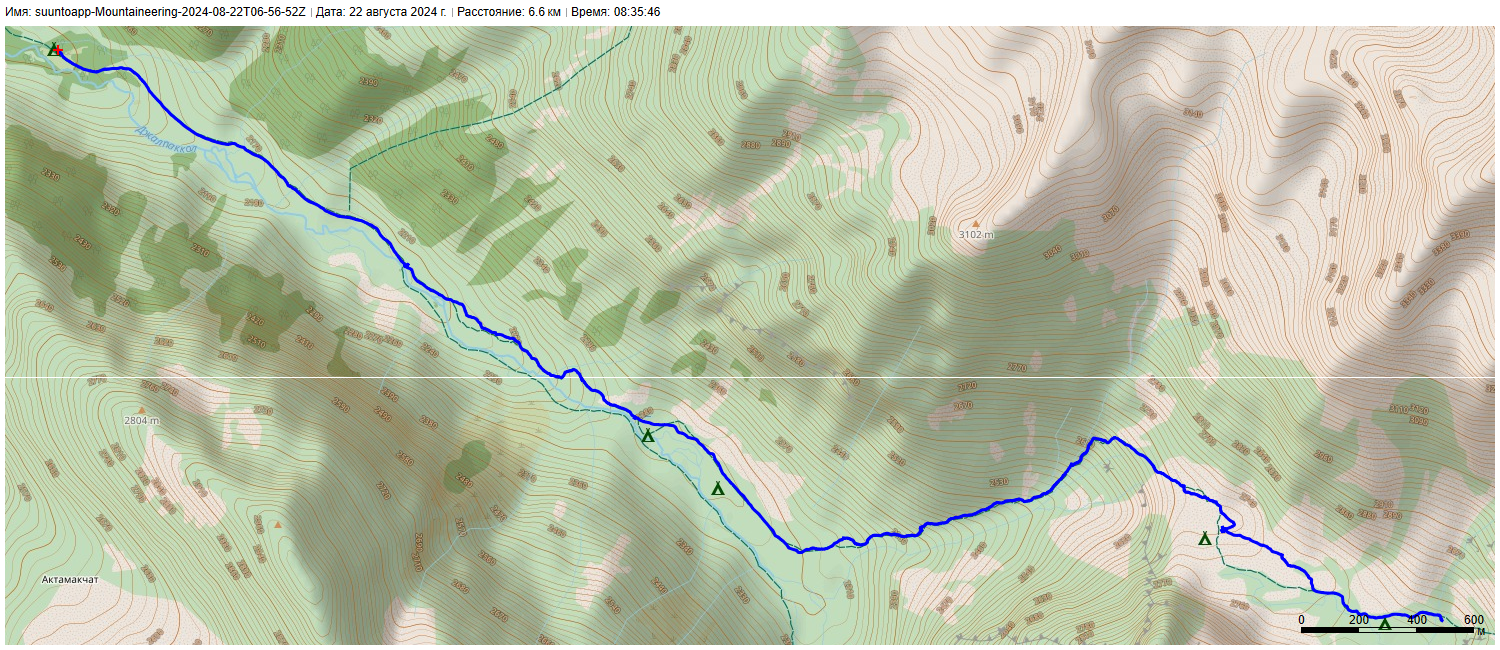
\includegraphics[width=\linewidth]{../pics/mini_maps/22}
		\end{column}
	\end{columns}
\end{frame}




\begin{frame}
	\frametitle{Крокусы в д.р. Джалпаккол}
	\framesubtitle{День 5, 22 августа}
	\footnotesize«Джалпак къол»~--- «Плоское ущелье»
	\centering
	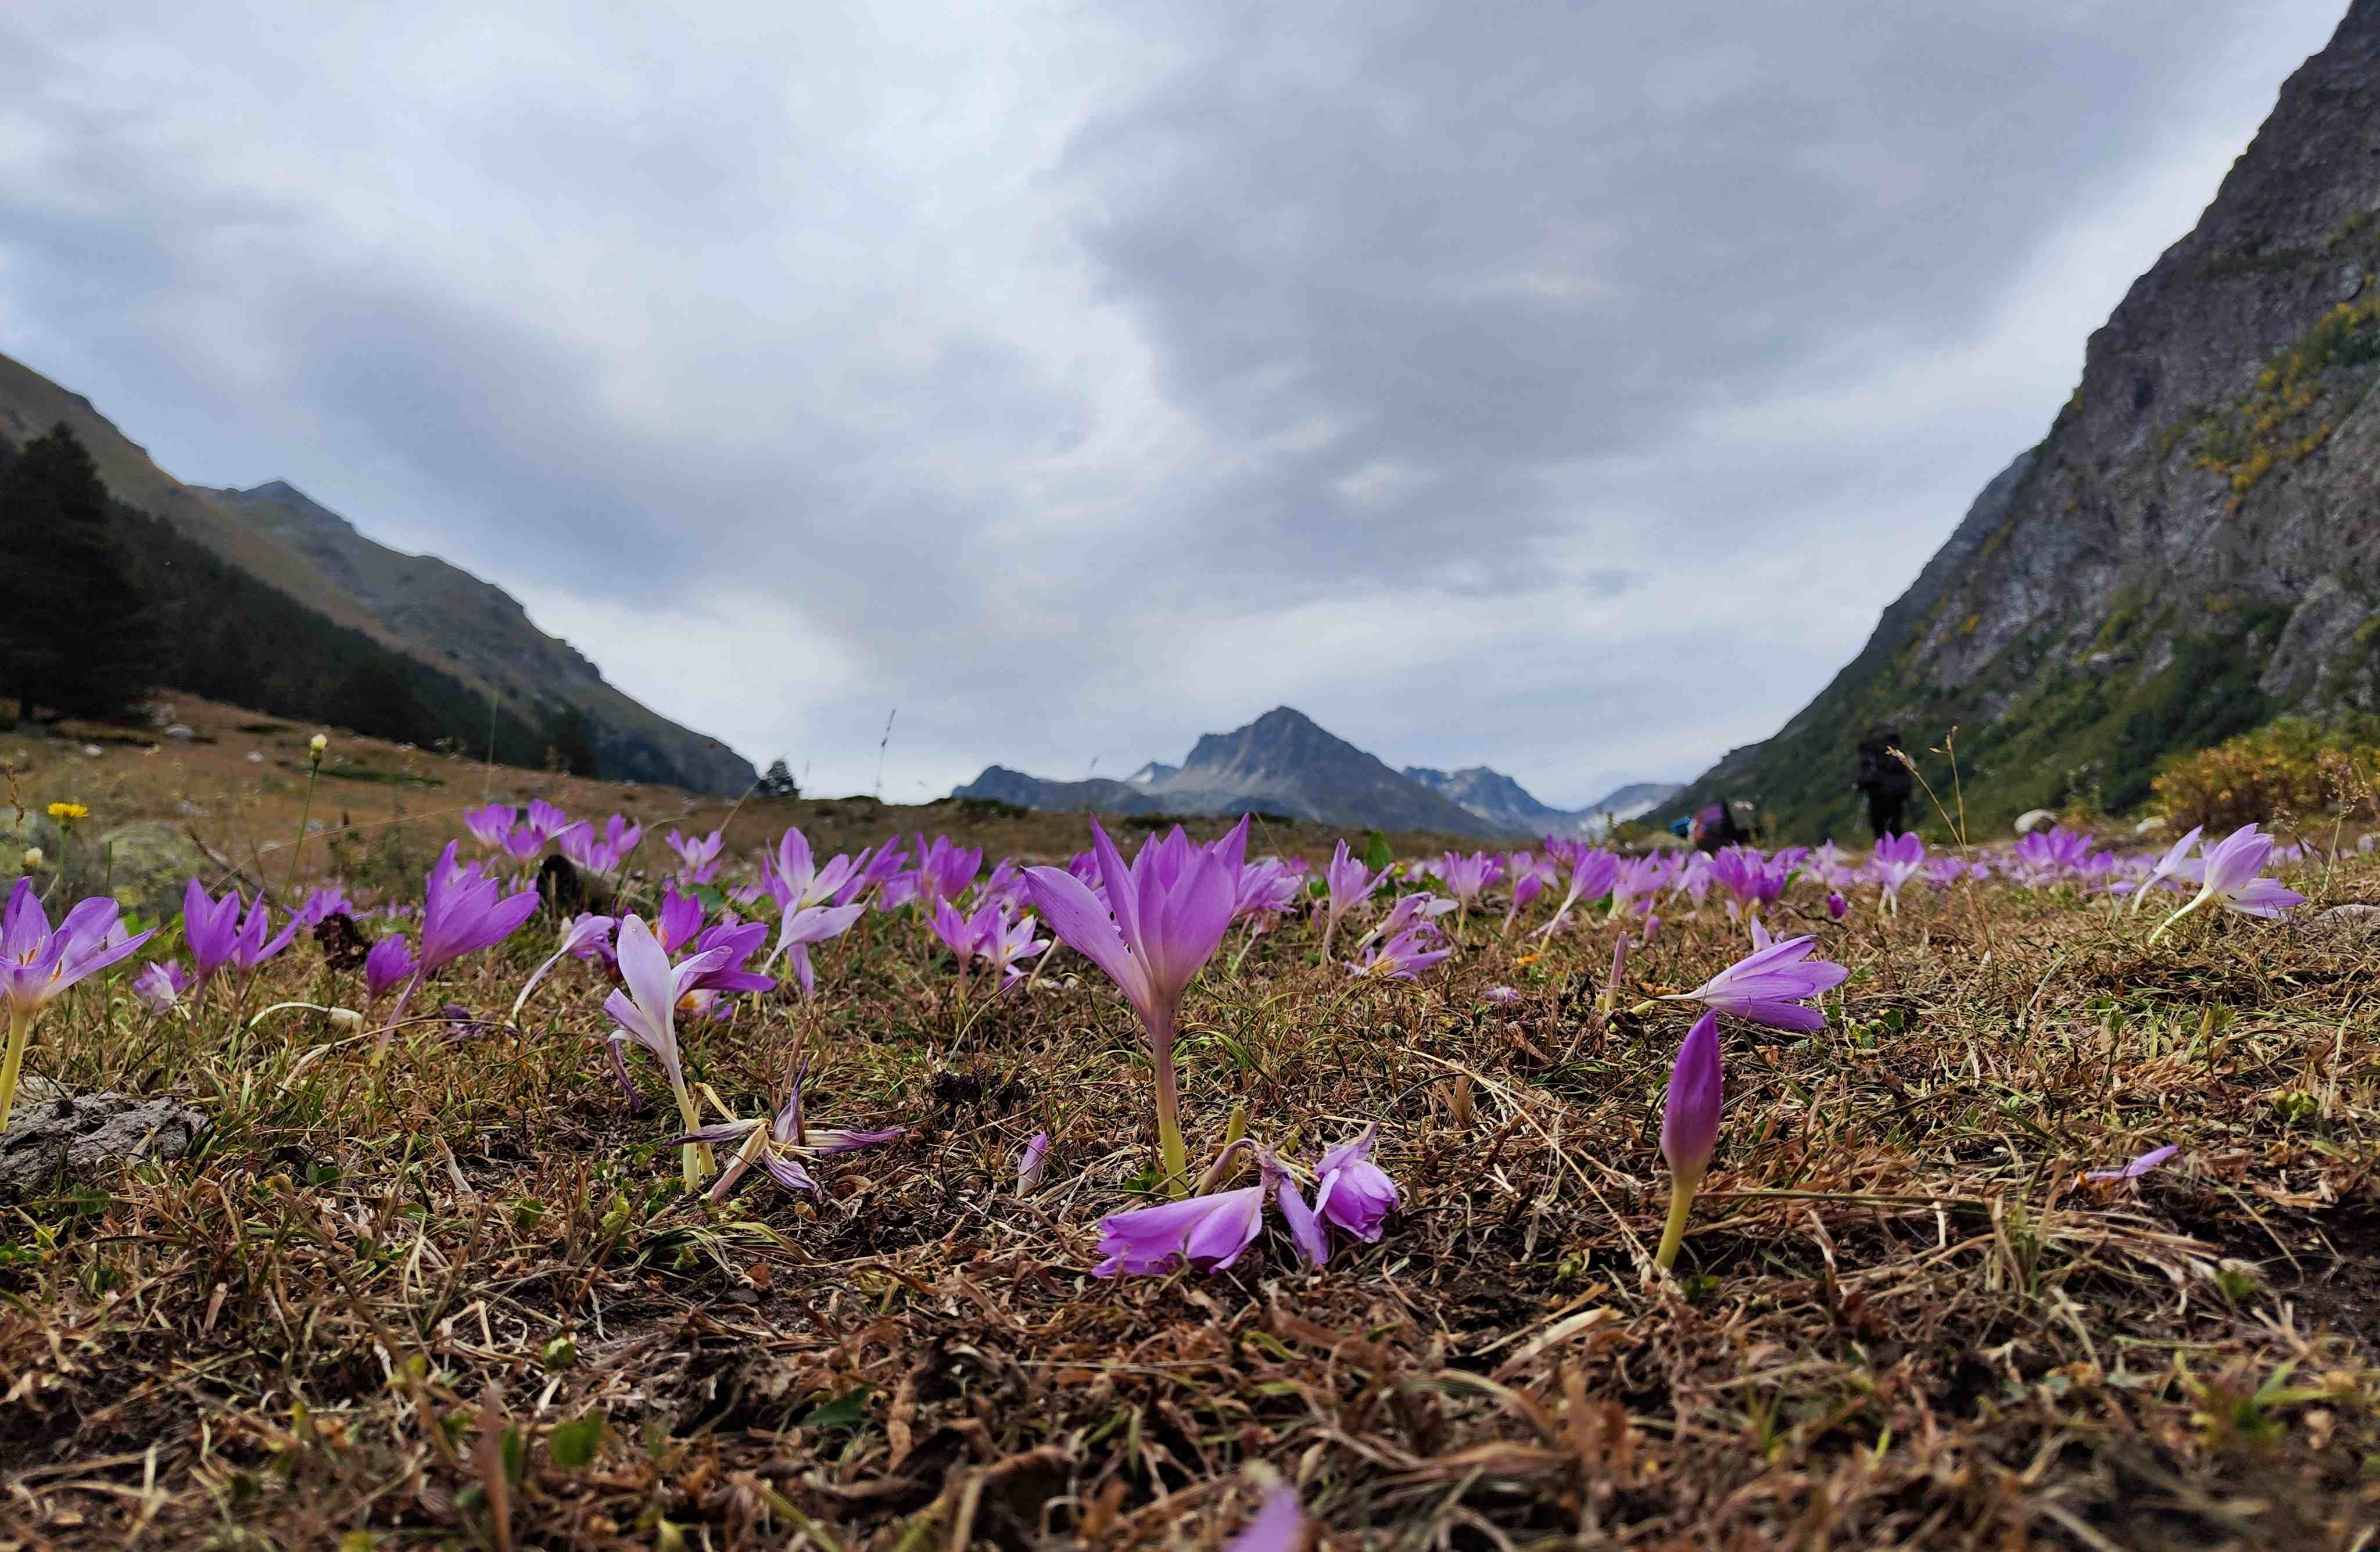
\includegraphics[width=0.9\textwidth]{../pics/IMG_20240822_101449}			
\end{frame}

\begin{frame}
	\frametitle{Поворот в д.р. Кичкинекол Джалпаккольский}
	\framesubtitle{День 5, 22 августа}
	\centering
	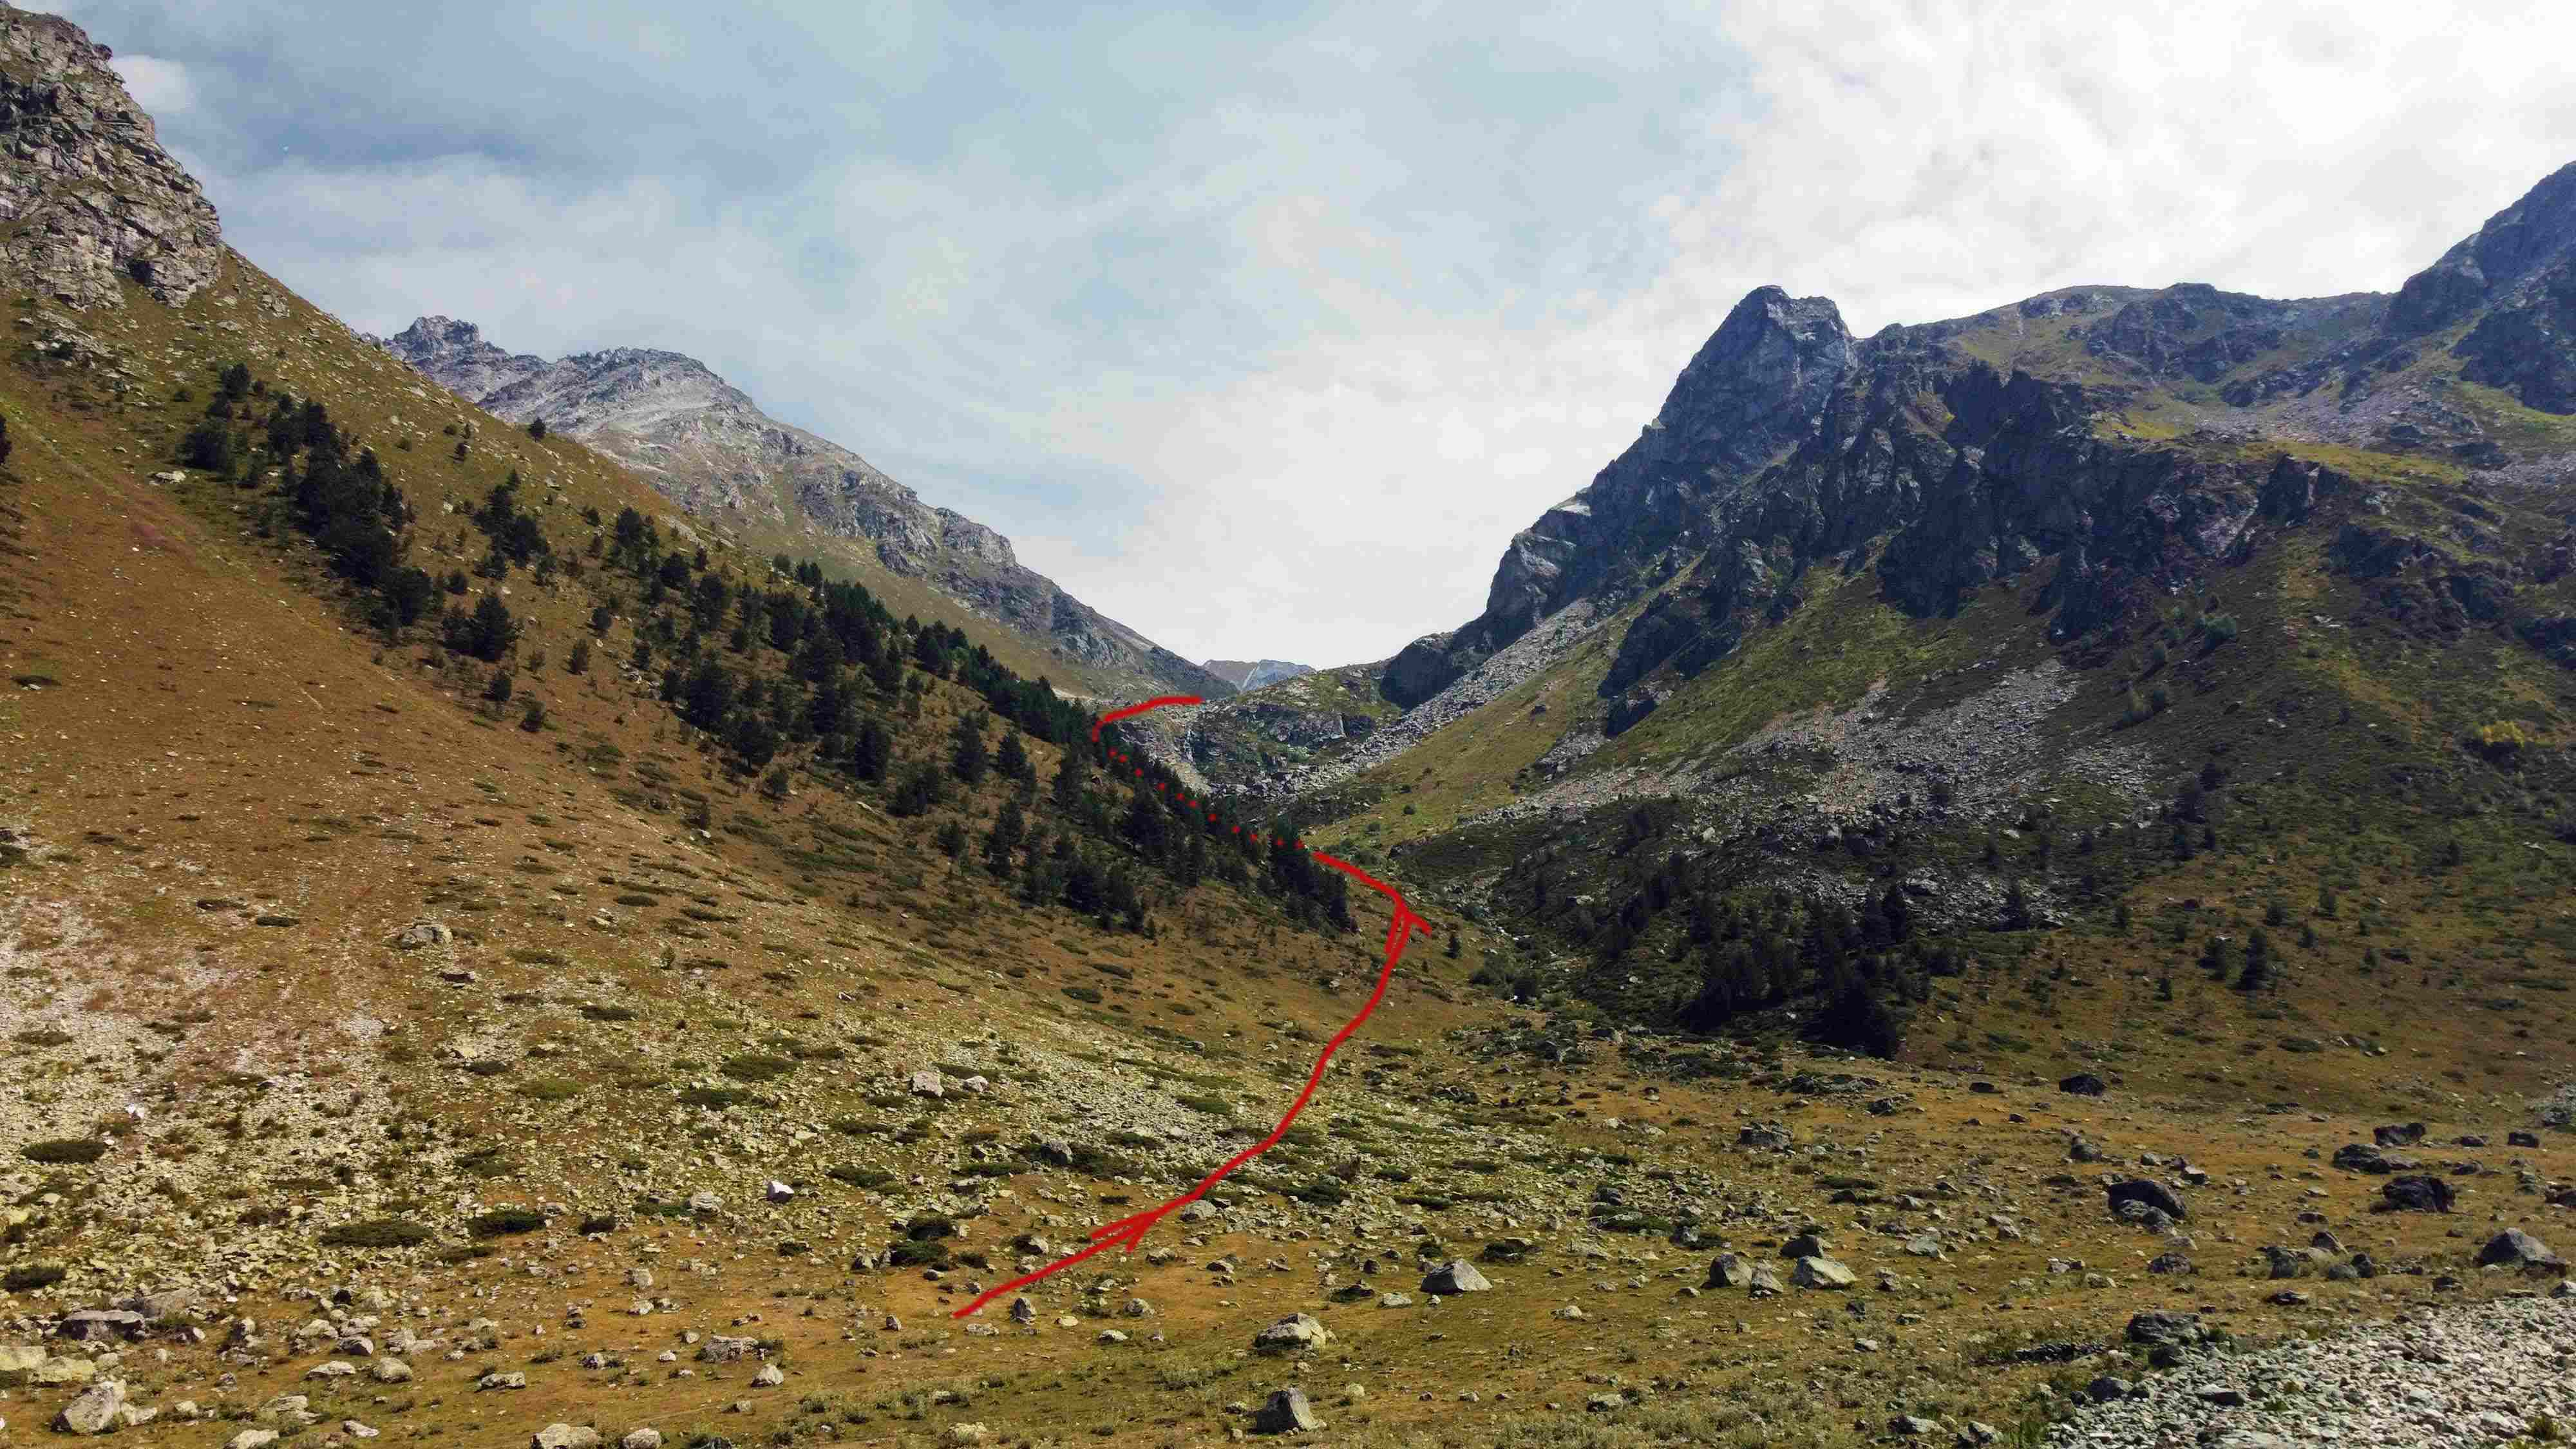
\includegraphics[width=\textwidth]{../pics/DJI_0835}			
\end{frame}



\begin{frame}
	\frametitle{\textAlpha\textpi \textomikron\textkappa\textalpha\textlambda\textnu\textpsi\textiota\textvarsigma}
	\framesubtitle{День 5, 22 августа}
	\centering
	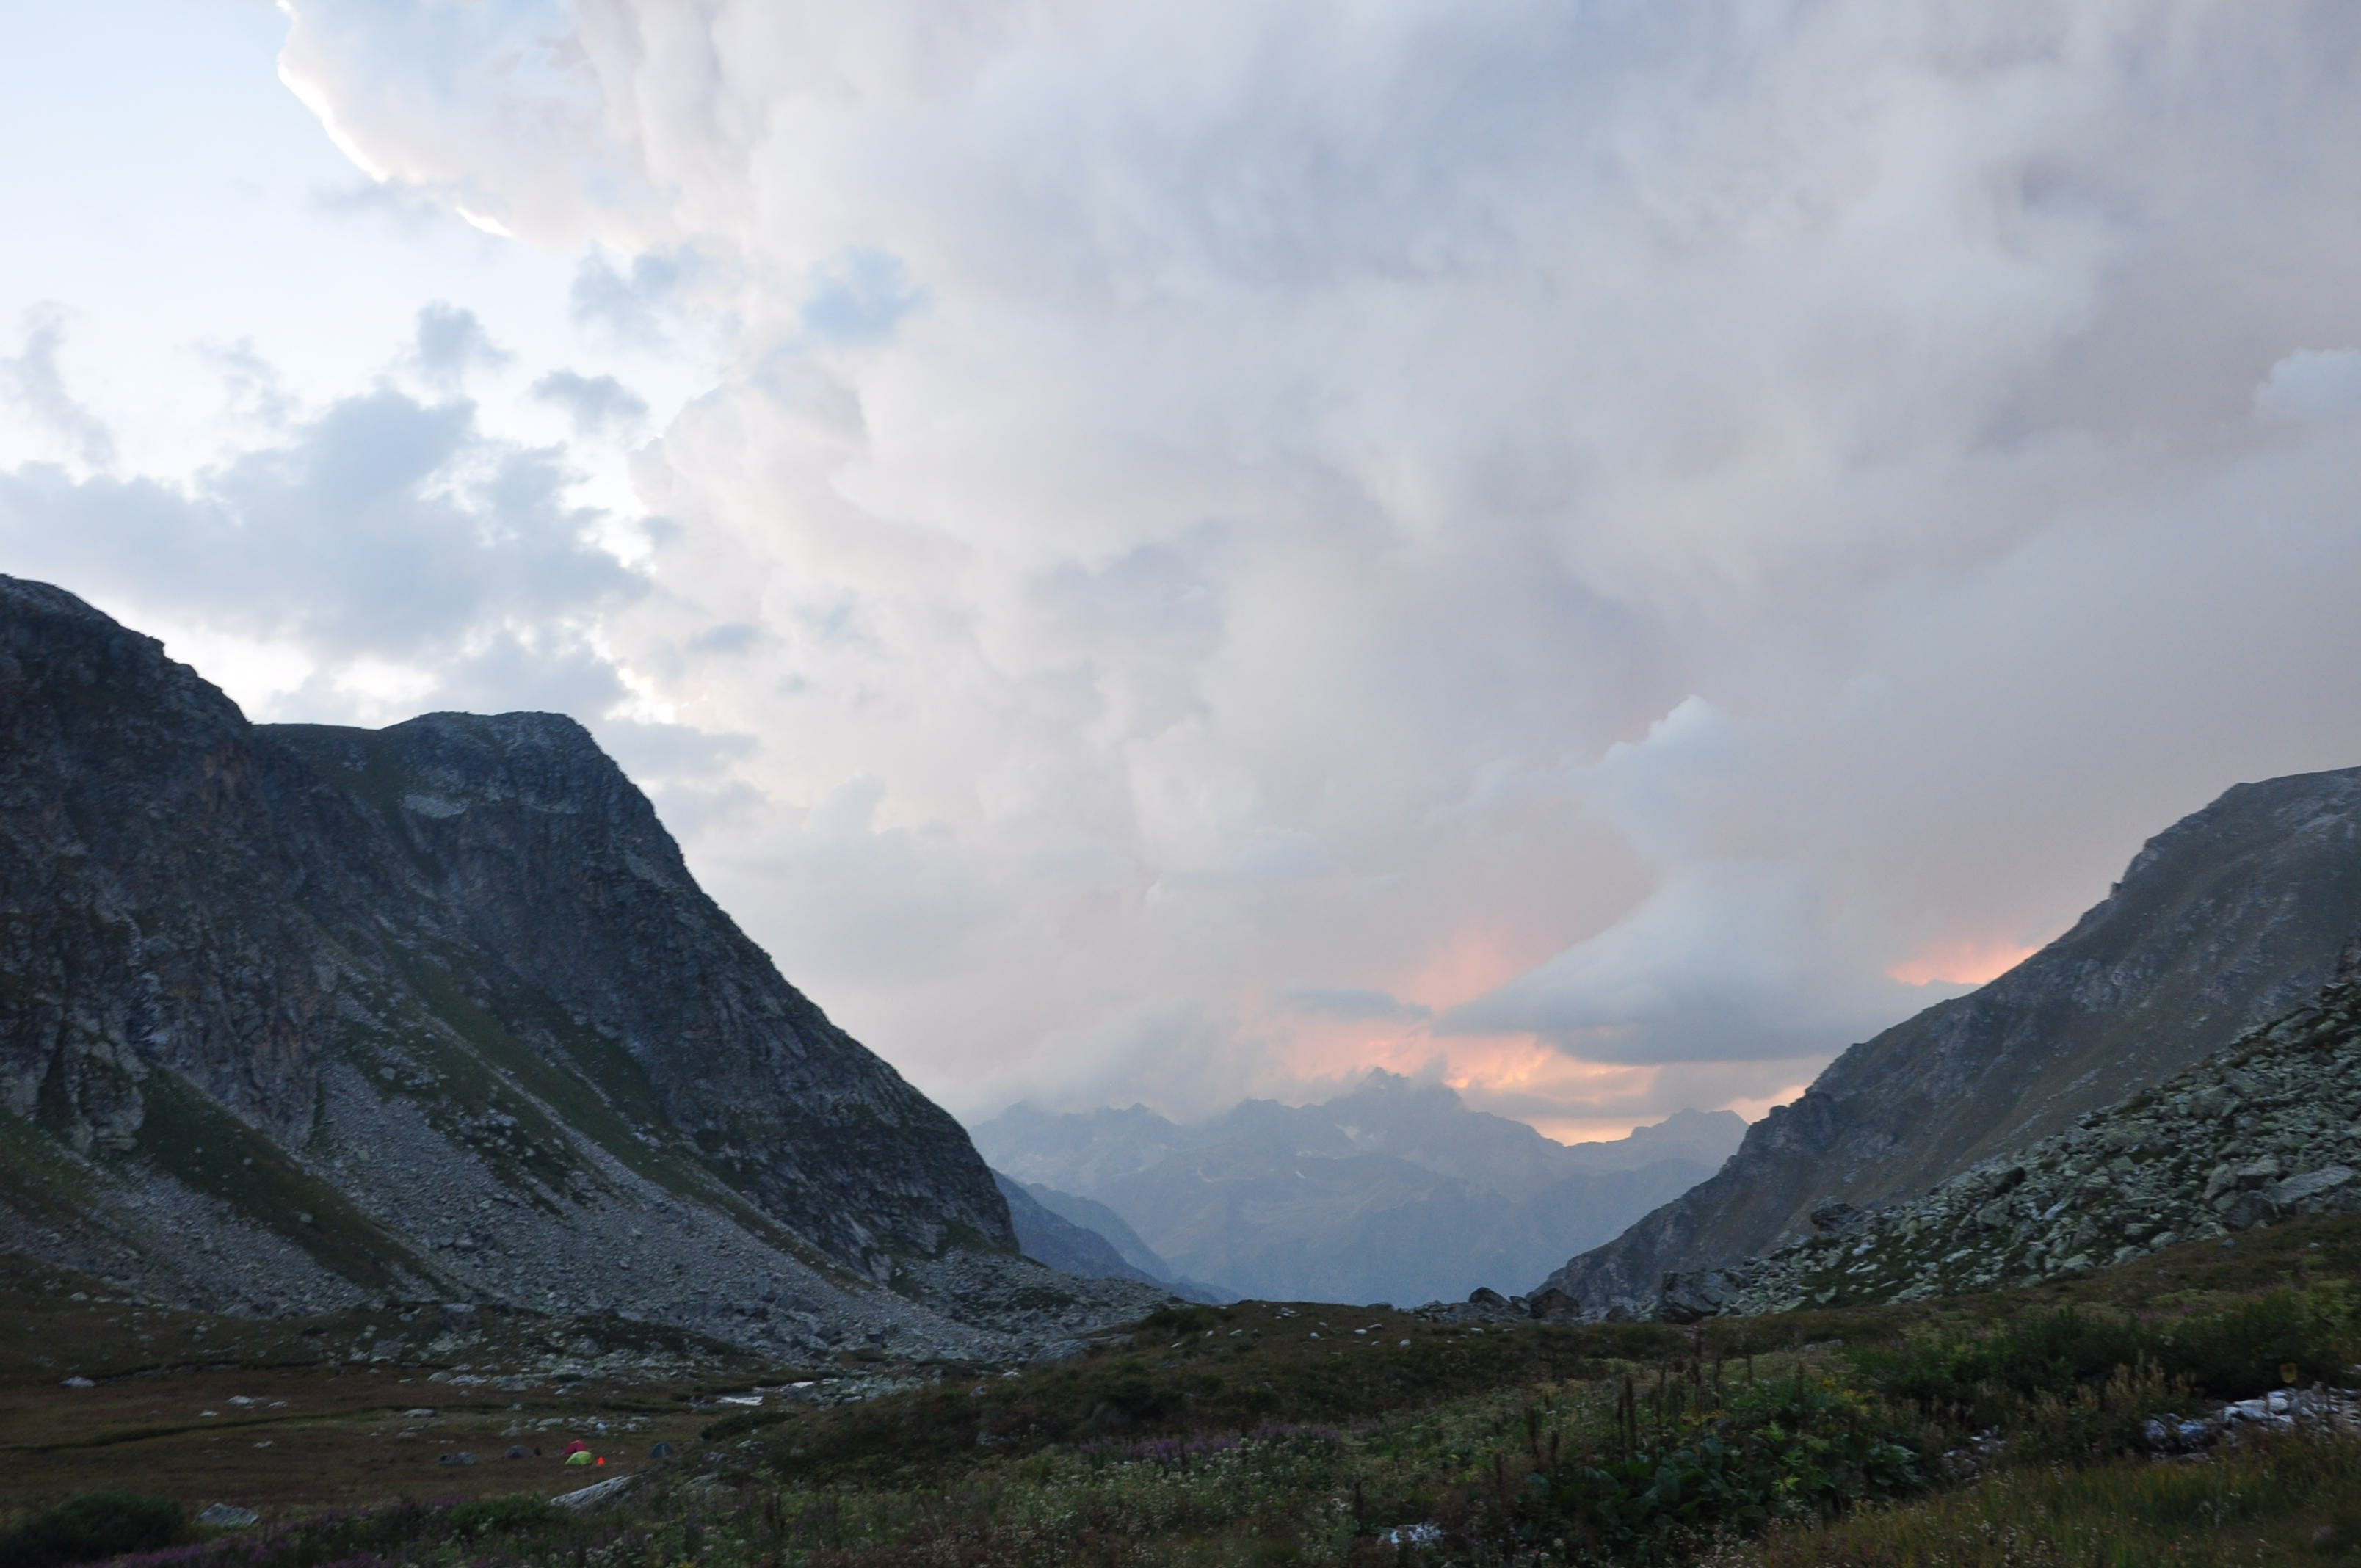
\includegraphics[width=\textwidth]{../pics/DSC_0010}			
\end{frame}
